\documentclass[conference]{IEEEtran}
\IEEEoverridecommandlockouts

\usepackage{cite}
\usepackage{amsmath,amssymb}
\usepackage{booktabs}
\usepackage{tabularx}
\usepackage{array}
\usepackage{graphicx}
\usepackage{xcolor}
\usepackage{url}
\usepackage[hidelinks]{hyperref}
\usepackage{tikz}
\usetikzlibrary{arrows.meta,positioning,shapes.geometric,fit}
\usepackage{enumitem}
\usepackage{balance}
\hypersetup{hidelinks}

\title{PFIV Guard: Website-Purpose-Aware Risk Assessment and Payment-Flow Integrity Verification}

\author{
\IEEEauthorblockN{Pranav Dwivedi, Aman Yadav, and Shourya Goyal}
\IEEEauthorblockA{School of Computer Science and Engineering (CSE), Business Systems\\
Vellore Institute of Technology, Vellore, India}
}

\begin{document}
\maketitle

\begin{abstract}
Phishing-risk tools can produce a single label without explaining what a webpage is intended to do or whether a payment-flow check is relevant to the inspected page. This paper presents PFIV Guard, an academic defensive prototype that combines explainable website-purpose detection with Payment Flow Integrity Verification (PFIV). A static-HTML heuristic module estimates page purpose and separately detects transaction intent. PFIV is conditionally applied to pages with transaction-specific evidence; ordinary informational pages, marketing homepages, and login-only forms are not treated as active checkout flows. When applicable, PFIV inspects sensitive form destinations, observed processor domains, redirects, embedded resources, and intermediary domains. The prototype also supports URL/HTML machine-learning analysis, screenshot OCR indicators, and QR/UPI payload decoding. On the saved UCI Phishing Websites held-out split, the Random Forest benchmark achieved 97.65\% accuracy, 98.03\% precision, 96.63\% recall, and 97.33\% F1; these figures do not represent live-web accuracy. Ten synthetic purpose/PFIV fixtures matched their expected outputs, and four controlled payment-flow fixtures matched their expected PFIV states. A four-case ablation changed three final decision categories when PFIV was included; this 75\% decision-change rate is not an accuracy measure. The prototype is not a production security service. Public deployment and participant-based usability testing remain pending; the paper reports analytical usability work and an implemented data-capture protocol without inventing participant results.
\end{abstract}

\begin{IEEEkeywords}
phishing assessment, payment security, payment-flow integrity, website purpose detection, explainable systems, QR analysis, usability evaluation
\end{IEEEkeywords}

\section{Introduction}
A user may encounter an unfamiliar page while shopping, booking a ticket, accessing online banking, or following a payment link. A generic phishing label does not necessarily explain the page's apparent function, whether the page is currently collecting payment data, or why an observed payment destination should be trusted or reviewed. Usability is defined in a specified context of use through effectiveness, efficiency, and satisfaction, rather than by the presence of functioning controls alone \cite{iso9241}.

PFIV Guard addresses two connected questions: (1) what does the inspected page appear to do, and (2) if the page appears to be in a transaction step, is the observable sensitive-payment path consistent with the processor claimed by the page? The second question is addressed through Payment Flow Integrity Verification (PFIV), the principal proposed technical contribution of this project. Website-purpose detection is a supporting context layer that determines whether PFIV should run; it is not a substitute for PFIV.

The project accepts a URL, a screenshot, or a QR-code image. Website URLs are fetched passively and analysed using static HTML. Screenshot input is processed using optical character recognition (OCR) and cautious heuristic indicators. QR input is decoded into either a web destination or a payment URI. A URL found in a screenshot or a web URL decoded from a QR code can be explicitly sent to the common URL-analysis pipeline. UPI payload fields are displayed for inspection only; the application does not initiate a payment.

The contributions of this report are:
\begin{itemize}[leftmargin=*]
    \item an explainable static-HTML Website Purpose and Functionality Detection (WPFD) layer that estimates a page category and visible functions;
    \item a separate transaction-intent gate that makes PFIV \emph{Not Applicable} when no active payment step is observed;
    \item a PFIV evidence branch that checks payment-specific form endpoints, processor consistency, redirects, embedded resources, and intermediary domains;
    \item integration of URL/HTML machine-learning output, screenshot/OCR evidence, and QR/UPI inspection in a common user-facing prototype; and
    \item a controlled fixture evaluation, ablation analysis, automated test suite, and a documented usability-study protocol.
\end{itemize}

The work does not claim that generic multimodal phishing detection, OCR, visual similarity, or processor identification alone is new. Prior systems such as Phishpedia and PhishIntention study visual identification and webpage intention using more advanced visual or dynamic approaches \cite{phishpedia,phishintention}. PFIV Guard is narrower and more transparent: it focuses on static, observable evidence along the sensitive-payment path, with explicit unknown and non-applicable states.

\section{Problem Definition and Threat Model}
\subsection{Problem}
An inspected domain can host different page types. A payment-gateway company's marketing homepage may describe payment services without collecting payment details. A login page may contain a username and password form but no payment transaction. Conversely, a checkout page may display a genuine processor brand while submitting sensitive fields to an unexpected endpoint. Therefore, page purpose and transaction intent must be evaluated separately.

\subsection{Threat scenario}
The motivating scenario is a deceptive checkout interface that presents a trusted processor name while routing sensitive payment information to an unexpected endpoint or intermediary. A processor appearing somewhere in a page does not, by itself, prove that the complete sensitive-data path is trustworthy. The proposed PFIV question is: can a user-side static inspection identify whether the observable sensitive-payment path is consistent with the processor claimed or expected by the page, and whether unexpected intermediary domains are visible?

\subsection{Scope and assumptions}
The current implementation inspects public HTTP/HTTPS responses using passive GET requests. It does not submit forms, authenticate to sites, execute browser JavaScript, or observe every runtime API request. The analysis is therefore limited to evidence available in the downloaded static HTML and HTTP redirect metadata. These constraints are important for interpreting both positive and negative findings.

\section{Related Work}
The UCI Phishing Websites dataset provides a tabular benchmark of URL and webpage-related features used for classification experiments \cite{uci}. Phishpedia compares webpage visual identity against known brand references to explain phishing identification \cite{phishpedia}. PhishIntention studies phishing intention using webpage appearance and dynamics, including interaction-based evidence \cite{phishintention}. These works demonstrate that webpage identity and intention are important signals, while also showing that the literature already contains visual and interaction-based phishing research. PFIV Guard does not claim novelty for those general directions. Its proposed contribution is the explicit transaction-intent gate and the PFIV evidence branch for static, observable payment-path consistency.

For usability, ISO 9241-11 provides the effectiveness, efficiency, and satisfaction framework \cite{iso9241}. The System Usability Scale (SUS) is a ten-item perceived-usability questionnaire \cite{sus}. The Keystroke-Level Model (KLM) predicts expert task time from low-level operators such as mental preparation, keystrokes, pointing, hand movement, and system response \cite{klm}. These methods provide complementary analytical and empirical evaluation routes; a KLM estimate is not a substitute for observing participants.

\section{System Architecture}
Fig.~\ref{fig:architecture} summarises the prototype. WPFD runs after page retrieval and before PFIV. URL/HTML machine-learning evidence is produced independently. Screenshot OCR and QR decoding are additional input paths. Available evidence is fused into an explainable risk assessment.

\begin{figure*}[t]
\centering
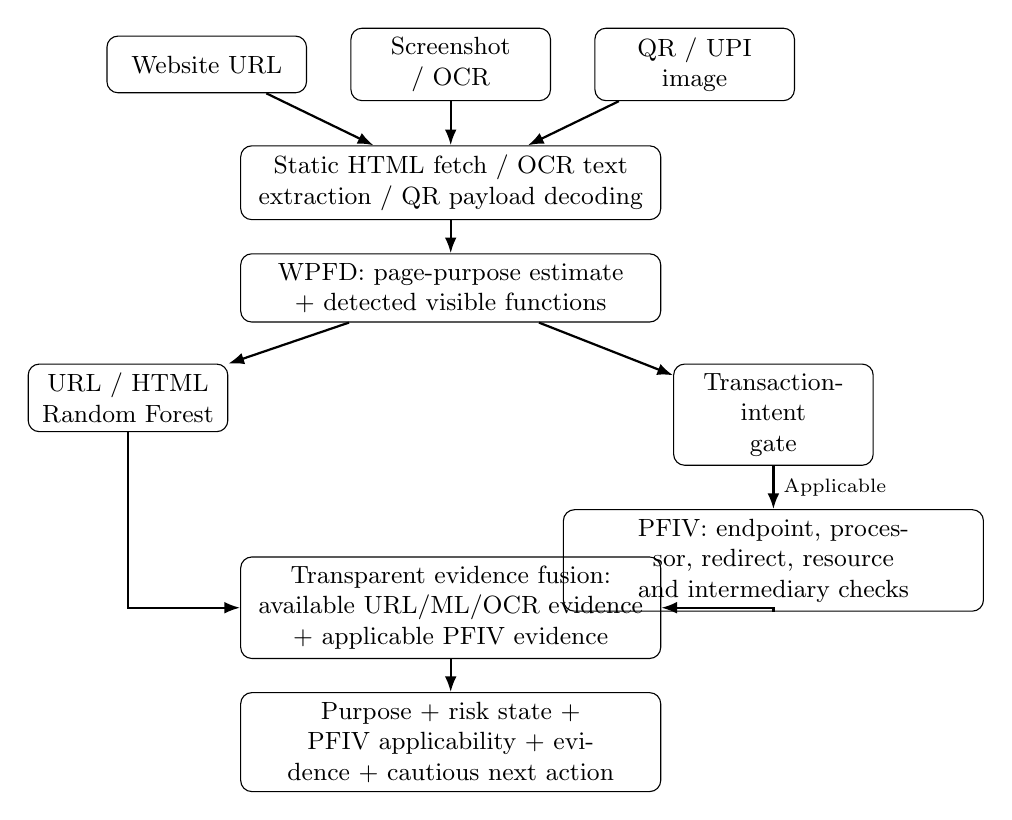
\begin{tikzpicture}[
  node distance=0.42cm and 0.55cm,
  box/.style={draw,rounded corners,align=center,minimum height=0.72cm,text width=2.3cm,font=\small},
  wide/.style={draw,rounded corners,align=center,minimum height=0.68cm,text width=5.1cm,font=\small},
  arr/.style={-{Latex[length=2mm]},thick}
]
\node[box] (url) {Website URL};
\node[box,right=of url] (shot) {Screenshot / OCR};
\node[box,right=of shot] (qr) {QR / UPI image};
\node[wide,below=0.56cm of shot] (extract) {Static HTML fetch / OCR text extraction / QR payload decoding};
\draw[arr] (url) -- (extract);
\draw[arr] (shot) -- (extract);
\draw[arr] (qr) -- (extract);
\node[wide,below=of extract] (wpfd) {WPFD: page-purpose estimate + detected visible functions};
\draw[arr] (extract) -- (wpfd);
\node[box,below left=0.52cm and 0.15cm of wpfd] (ml) {URL / HTML\\Random Forest};
\node[box,below right=0.52cm and 0.15cm of wpfd] (gate) {Transaction-intent\\gate};
\draw[arr] (wpfd) -- (ml);
\draw[arr] (wpfd) -- (gate);
\node[wide,below=0.55cm of gate] (pfiv) {PFIV: endpoint, processor, redirect, resource and intermediary checks};
\draw[arr] (gate) -- node[right,font=\scriptsize]{Applicable} (pfiv);
\node[wide,below=0.52cm of wpfd,yshift=-2.45cm] (fusion) {Transparent evidence fusion: available URL/ML/OCR evidence + applicable PFIV evidence};
\draw[arr] (ml.south) |- (fusion.west);
\draw[arr] (pfiv.south) |- (fusion.east);
\node[wide,below=of fusion] (report) {Purpose + risk state + PFIV applicability + evidence + cautious next action};
\draw[arr] (fusion) -- (report);
\end{tikzpicture}
\caption{Purpose-aware PFIV Guard architecture. PFIV is not run for pages without observed transaction-specific intent.}
\label{fig:architecture}
\end{figure*}

\subsection{Website Purpose and Functionality Detection}
WPFD analyses the inspected page's title, meta description, headings, visible controls, forms, URL path, and a bounded sample of body text. The current rule-based categories include informational/knowledge, e-commerce, banking/financial services, payment gateway/FinTech, booking/reservations, productivity/SaaS, education, news/media, government, healthcare, other, and unknown. Detected functions may include authentication, search, product browsing/cart, booking, checkout/payment action, forms, and content reading.

The classifier uses evidence-source weights: title (5.0), headings (4.0), description (3.0), action text (3.0), form metadata (2.0), URL path (1.25), and body text (0.35). Phrase matches accumulate category scores; the leading category and the separation from the next category produce a heuristic evidence-strength indicator. This indicator is not a calibrated probability and cannot authenticate a website owner or establish that a page is safe. If the evidence is weak, the result is ``Unknown / Insufficient Evidence.''

\subsection{Transaction-Intent Gate}
WPFD and transaction intent are separate outputs. The gate distinguishes active transaction evidence from generic wording. PFIV is triggered by a payment-specific form; an explicit payment-action control combined with transaction context; or a checkout/payment route combined with transaction context. Generic wording such as “payment gateway”, “accept payments”, or “online payments” is insufficient by itself. A general username/password login form is not treated as a payment form. When only generic payment wording is present, the page can be marked as potential payment-related content while PFIV remains Not Applicable. The full PFIV scoring and processor-path inspection is not invoked for such pages.

\subsection{Payment Flow Integrity Verification}
When transaction intent is detected, PFIV examines:
\begin{itemize}[leftmargin=*]
  \item payment-specific form fields and form action destinations;
  \item claimed processor names visible in the page and processor domains observed in form actions, redirects, iframes, or scripts;
  \item external sensitive-data endpoints and unexpected intermediary domains; and
  \item whether enough static evidence exists to establish the sensitive-payment path.
\end{itemize}

The processor reference registry is local and finite (e.g., Razorpay, Stripe, PayPal, PayU, Cashfree, PhonePe, CCAvenue, BillDesk, and Adyen). Its coverage may be incomplete or outdated. A path is labelled Verified only when a payment-specific form endpoint is on a known processor domain, the processor evidence is consistent with the page's claim, and no suspicious external or intermediary domains are observed. A processor found only in a script or iframe without an established sensitive form endpoint is not sufficient to claim verification.

The current PFIV evidence score uses configured rules: an unexpected external sensitive endpoint adds 30; a processor mismatch adds 55; an unidentified processor on a payment page adds 15; and unexpected intermediary domains add 20. A transaction page whose sensitive path cannot be established is Unverifiable with score 35. Scores of 50 or more produce Suspicious; lower non-zero scores produce Needs Review. Verified, Suspicious, Unverifiable, Needs Review, and Not Applicable are distinct outcomes. Not Applicable means the inspected page did not show a strong active transaction step, not that the entire website is safe.

\subsection{Evidence Fusion and Other Inputs}
The fusion layer combines available URL, ML, OCR indicator, and PFIV evidence using configured weights (URL 0.25, visual 0.10, PFIV 0.30, threat intelligence 0.10, ML 0.25), normalised over branches that actually supplied evidence. Missing or inactive evidence is passed as unavailable rather than as a zero-risk observation. A suspicious PFIV result imposes a conservative high-risk floor. The weights are configured, not learned by a meta-classifier.

The URL/HTML branch applies a Random Forest model through a live feature adapter. The original model was trained on the UCI phishing benchmark; some historic features, such as web traffic or page rank, are not reliably observable for arbitrary live pages. Live output is therefore indicative and not calibrated live-web accuracy. SHAP artifacts are associated with the URL/HTML model branch. Screenshot processing extracts visible text, possible URLs, payment-related terms, and urgency indicators using OCR; no trained screenshot/logo classifier is present. QR decoding uses OpenCV; a web URL can be explicitly analysed, while UPI URI fields are displayed without initiating payment or verifying the payee.

\section{Implementation and Safety Controls}
The application is implemented in Python with Streamlit. URL handling, static HTML parsing, page-purpose classification, PFIV, evidence fusion, screenshot OCR, QR decoding, model output, and a facilitated user-study data-capture tab are separate modules. Public HTTP requests use bounded timeouts, a response-size limit, and a redirect limit. Local, private, loopback, link-local, and reserved targets are blocked by default; a narrow local fixture bypass is available only in explicit development mode. These controls reduce risk but do not constitute an external security audit. SSRF is a recognised risk when a server fetches user-supplied URLs; application- and network-layer controls are recommended by OWASP \cite{owasp}.

The deployment package includes a Streamlit Community Cloud dependency manifest, a Linux package manifest for Tesseract, a CI workflow, and an alternative Dockerfile. Community Cloud requires Python dependencies in a requirements file and external Linux packages in packages.txt when needed \cite{streamlitdeps}; deployment requires a connected repository and an explicit deployment action \cite{streamlitdeps}. No public deployment URL is included in this report. The app has not been independently penetration-tested and should remain an academic demonstration, not an unrestricted production URL-fetching service.

\section{Experimental Setup}
\subsection{Offline Phishing Benchmark}
The Random Forest and Logistic Regression models were evaluated on the UCI Phishing Websites dataset (UCI ID 327), which contains 11,055 instances and 30 integer features, with no missing values in the supplied dataset description \cite{uci}. The implementation applies an 80/20 stratified train/test split with random state 42: 8,844 training rows and 2,211 test rows. Logistic Regression uses a standardisation pipeline and a maximum of 2,000 iterations. The Random Forest uses 300 trees, balanced class weights, all available CPU jobs, and random state 42. The held-out split results are reported in Table~\ref{tab:ml}.

\begin{table}[t]
\caption{Offline UCI Test-Split Results}
\label{tab:ml}
\centering
\scriptsize
\begin{tabular}{lrrrr}
\toprule
Model & Acc. & Prec. & Recall & F1 \\
\midrule
Logistic Regression & 92.81 & 93.44 & 90.10 & 91.74 \\
Random Forest & 97.65 & 98.03 & 96.63 & 97.33 \\
\bottomrule
\end{tabular}
\vspace{1mm}
\parbox{\columnwidth}{\scriptsize Values are percentages. These are held-out UCI split metrics, not accuracy on arbitrary live websites.}
\end{table}

For Random Forest, the saved confusion matrix is TN=1212, FP=19, FN=33, and TP=947 (rows: actual class; columns: predicted class, with legitimate as class 0 and phishing as class 1). The live feature adapter maps observable URL/HTML signals into the benchmark-compatible feature schema; several original features are unavailable or approximated during live inspection. The benchmark should therefore not be represented as an end-to-end live website detection evaluation.

\subsection{Purpose and PFIV Fixture Validation}
A deterministic offline validator runs ten synthetic HTML fixtures. Six cover non-transaction page contexts (informational, e-commerce catalogue, banking homepage, payment-gateway marketing homepage, booking page, and login form); four cover controlled payment-flow scenarios (legitimate, external attacker endpoint, processor mismatch, and unverifiable checkout). The test compares expected and observed purpose category, transaction-intent status, and PFIV outcome. All ten fixtures matched their expected states (10/10). This result verifies implemented rules against designed fixtures; it is not a real-world purpose-classification accuracy measure.

\begin{table}[t]
\caption{Four Controlled PFIV Scenarios}
\label{tab:pfiv}
\centering
\scriptsize
\begin{tabularx}{\columnwidth}{@{}Xlll@{}}
\toprule
Scenario & Expected & Observed & PFIV score \\
\midrule
Legitimate payment path & Verified & Verified & 0 \\
External attacker endpoint & Suspicious & Suspicious & 65 \\
Processor mismatch & Suspicious & Suspicious & 55 \\
Unverifiable payment path & Unverifiable & Unverifiable & 35 \\
\bottomrule
\end{tabularx}
\vspace{1mm}
\parbox{\columnwidth}{\scriptsize All four controlled fixture states matched. The score is rule-based evidence scoring, not a probability.}
\end{table}

\subsection{PFIV Ablation}
The ablation compares the full system with a baseline that removes PFIV. In this evaluation no screenshot was supplied and no live threat-intelligence feed was available; those branches are treated as unavailable, not as zero-risk observations. The baseline therefore renormalises the available URL and ML weights. Table~\ref{tab:ablation} shows that three of four controlled scenario decisions changed when PFIV was included. This is a four-fixture decision-change rate, not model accuracy, recall, or a statistically generalisable estimate.

\begin{table*}[t]
\caption{PFIV Ablation on the Four Controlled Scenarios}
\label{tab:ablation}
\centering
\scriptsize
\begin{tabular}{lrrrrll}
\toprule
Scenario & Baseline score & Baseline label & Full score & Full label & PFIV state & Decision changed \\
\midrule
Legitimate payment path & 24.55 & Legitimate & 15.34 & Legitimate & Verified & No \\
External attacker endpoint & 24.78 & Legitimate & 65.00 & High Risk & Suspicious & Yes \\
Processor mismatch & 24.55 & Legitimate & 65.00 & High Risk & Suspicious & Yes \\
Unverifiable payment path & 23.98 & Legitimate & 35.00 & Suspicious & Unverifiable & Yes \\
\bottomrule
\end{tabular}
\end{table*}

\subsection{Automated Software Tests}
The updated source test suite reports 29 passing tests in the current preparation environment. It covers URL input validation, narrow local-fixture allowlisting, payment-versus-credential form handling, QR decoding, screenshot input/OCR handling, fusion safeguards, website-purpose classification, transaction-intent gating, PFIV fixture outcomes, and SUS scoring helpers. Automated software tests establish only the behaviours covered by those tests; they do not demonstrate usability or broad real-world security performance.

\section{Usability Evaluation}
The interface is organised around the user journey: choose an input, submit or decode it, interpret website purpose and evidence, understand whether PFIV applies, and choose a safe next action. A preliminary single-reviewer heuristic inspection and analytical task decomposition were documented. The current prototype also includes a facilitated user-study tab that records anonymous task success, time, errors, help requests, and ten SUS responses. Study data remain in the active application session and must be exported by the facilitator after each session.

An illustrative KLM task models a user pasting a URL and analysing it. With assumed operator values $M=1.35$ s, $P=1.10$ s, $K=0.28$ s, $H=0.40$ s, and one assumed response time $R=0.84$ s, the paste sequence (2M, 2P, 4K, 2H, 1R) gives:
\begin{equation}
T_{paste}=2M+2P+4K+2H+R=7.66\text{ s}.
\end{equation}
For typing a 26-character URL, two pointing clicks and 26 typed characters give 28K operators, resulting in:
\begin{equation}
T_{type}=2M+2P+28K+2H+R=14.38\text{ s}.
\end{equation}
These are assumption-based expert performance estimates, not participant timings; the response-time component is variable with network and server conditions. KLM is therefore used as a design comparison, not as empirical evidence of user performance.

No participant sessions or SUS responses were included with the uploaded project at the time of this report. Consequently, user task-completion rates, observed times, error rates, help rates, warning comprehension, and group SUS statistics are not reported. The study protocol recommends voluntary adult participants, anonymous codes, synthetic or benign tasks, informed consent, and no collection of credentials or payment data. A small convenience sample can support formative iteration but cannot establish population-wide usability. Accessibility checks for keyboard access, visible focus, 200\% zoom, mobile reflow, colour contrast, and screen-reader status feedback remain to be completed in the deployed target environment.

\section{Discussion}
The purpose-aware gate addresses an important interpretability problem: a page that markets payment services is not necessarily a checkout page, and a login form is not necessarily a payment form. During a public Razorpay homepage check in an earlier build, generic marketing wording incorrectly caused transaction intent to be marked as detected even though the page exposed no sensitive payment form or payment iframe. The gate was tightened to require a payment-specific form, an explicit payment-action control with transaction context, or a checkout/payment route with transaction context. The synthetic payment-gateway marketing fixture now yields POTENTIAL with PFIV Not Applicable, and a regression test verifies that full PFIV scoring is not invoked for that case. The public Razorpay page must still be rechecked after the gate change on the target deployment. The ten synthetic fixture checks support the implemented separation of website purpose, transaction intent, and PFIV applicability. The controlled PFIV evaluation demonstrates that the rule set can distinguish the four designed states, while the ablation indicates that PFIV materially changed three of those four decisions.

The main limitations are substantial. WPFD is a rule-based static-HTML heuristic rather than a trained website-purpose classifier. Its evidence-strength value is not a calibrated probability. Static inspection may miss JavaScript-rendered forms, browser runtime requests, dynamically loaded payment widgets, and client-side redirects. The processor registry is finite. The live Random Forest adapter approximates some benchmark features that are not consistently observable from current webpages. The screenshot branch uses OCR heuristics rather than a trained computer-vision model. Live VirusTotal, PhishTank, OpenPhish, or equivalent threat-intelligence feeds are not connected. A normal page can still be misclassified by URL/ML or evidence fusion; results should be interpreted with the displayed evidence and limitations rather than as a definitive safe/unsafe verdict. The bundled Random Forest artifact was serialized with scikit-learn 1.6.1. The final ablation rerun in the preparation container emitted a version-mismatch warning because that container uses scikit-learn 1.8.0. Therefore, the displayed model-dependent ablation risk scores are provisional until regenerated in the pinned 1.6.1 environment; the fixture PFIV state comparisons are rule-based.

Public deployment configuration has been prepared, but no hosted URL is available in this project snapshot. Before wider public access, the URL-fetching service requires an independent SSRF and network-egress review, robust rate limiting and abuse monitoring, and post-deployment smoke testing. The deployment files are a packaging step, not proof of a completed deployment. Similarly, a user-study capture form is not proof that a user study has been conducted.

\section{Conclusion and Future Work}
This report presents PFIV Guard, a website-risk prototype that adds website-purpose estimation and transaction-intent gating around a static payment-flow integrity branch. It integrates a UCI-trained URL/HTML Random Forest, screenshot OCR indicators, QR/UPI decoding, purpose-aware PFIV, and explainable evidence presentation. The saved offline benchmark achieved 97.65\% Random Forest accuracy on the UCI held-out split, while ten synthetic purpose/PFIV fixtures and four controlled PFIV cases matched their expected outputs. In the designed ablation set, PFIV changed three of four final decision categories. None of these results establishes live-web accuracy or production security.

Future work includes (1) evaluating WPFD on a labelled, independently collected set of real page categories; (2) strengthening transaction-flow visibility through browser instrumentation in a controlled environment; (3) extending and validating the processor reference registry; (4) integrating reputable threat-intelligence feeds with documented rate limits and provenance; (5) completing an external SSRF/security review before public deployment; and (6) conducting participant-based usability testing and accessibility validation, then iterating the interface using measured task and SUS outcomes.

\section*{Data and Implementation Availability}
The project archive contains the Python source, model artifacts, synthetic HTML fixtures, unit tests, saved benchmark outputs, PFIV evaluation scripts, deployment configuration, and usability-study protocol. The present report does not include participant data because no real-user study records were available. The paper is an IEEE conference-style academic report; it is not an IEEE-published or peer-reviewed article.

\balance
\begin{thebibliography}{99}

\bibitem{uci}
R. Mohammad and L. McCluskey, ``Phishing Websites,'' UCI Machine Learning Repository, dataset 327, 2015, doi: 10.24432/C51W2X.

\bibitem{phishpedia}
Y. Lin, R. Liu, D. M. Divakaran, J. Y. Ng, Q. Z. Chan, Y. Lu, Y. Si, F. Zhang, and J. S. Dong, ``Phishpedia: A Hybrid Deep Learning Based Approach to Visually Identify Phishing Webpages,'' in Proc. 30th USENIX Security Symposium, 2021, pp. 3793--3810.

\bibitem{phishintention}
R. Liu, Y. Lin, X. Yang, S. H. Ng, D. M. Divakaran, and J. S. Dong, ``Inferring Phishing Intention via Webpage Appearance and Dynamics: A Deep Vision Based Approach,'' in Proc. 31st USENIX Security Symposium, 2022, pp. 1633--1650.

\bibitem{iso9241}
International Organization for Standardization, ``ISO 9241-11:2018: Ergonomics of Human-System Interaction -- Part 11: Usability: Definitions and Concepts,'' 2018.

\bibitem{sus}
J. Brooke, ``SUS: A quick and dirty usability scale,'' in \emph{Usability Evaluation in Industry}, P. W. Jordan, B. Thomas, I. L. McClelland, and B. Weerdmeester, Eds. London, U.K.: Taylor \& Francis, 1996, pp. 189--194.

\bibitem{klm}
S. K. Card, T. P. Moran, and A. Newell, ``The Keystroke-Level Model for User Performance Time with Interactive Systems,'' \emph{Communications of the ACM}, vol. 23, no. 7, pp. 396--410, 1980, doi: 10.1145/358886.358895.

\bibitem{owasp}
OWASP Foundation, ``Server-Side Request Forgery Prevention Cheat Sheet,'' OWASP Cheat Sheet Series. [Online]. Available: \url{https://cheatsheetseries.owasp.org/cheatsheets/Server_Side_Request_Forgery_Prevention_Cheat_Sheet.html}. Accessed: Oct. 31, 2026.

\bibitem{streamlitdeps}
Streamlit, ``Streamlit Community Cloud Documentation: App Dependencies and Deployment,'' [Online]. Available: \url{https://docs.streamlit.io/deploy/streamlit-community-cloud/deploy-your-app/app-dependencies} and \url{https://docs.streamlit.io/deploy/streamlit-community-cloud/deploy-your-app/deploy}. Accessed: Oct. 31, 2026.

\end{thebibliography}
\end{document}
